\documentclass[pdflatex,compress]{beamer}

%\usetheme[dark,framenumber,totalframenumber]{ElektroITK}
\usetheme[darktitle,framenumber,totalframenumber]{ElektroITK}
\usepackage{graphicx}
\usepackage{multicol}

\title{Data Communications}
\subtitle{Chapter 2 - Protocol Architecture}

\author{Mifta Nur Farid, M.T.}

\begin{document}

\maketitle

\begin{frame}
	\frametitle{The Need for a Protocol Architecture}
	To transfer data several tasks must be performed:
	\begin{enumerate}
		\item The source must either activate the direct communications path or inform the network of the identity of the desired destination system
		\item The source system must ascertain that the destination system is prepared to receive data
		\item The file transfer application on the source system must ascertain that the file management program on the destination system is prepared to accept and store the file for this particular user
		\item A format translation function may need to be performed by one or the other system if the file formats used on the two systems are different
	\end{enumerate}
\end{frame}

\begin{frame}
	\frametitle{Functions of Protocol Architecture}
	\begin{itemize}
		\item Breaks logic into subtask modules which are implemented separately
		\item Modules are arranged in a vertical stack
		\begin{itemize}
			\item Each layer in the stack performs a subset of functions
			\item Relies on next lower layer for primitive functions
			\item Provides services to the next higher layer
			\item Changes in one layer should not require changes in other layers
		\end{itemize}
	\end{itemize}
\end{frame}

\begin{frame}
	\frametitle{Key Features of a Protocol}
	\begin{itemize}
		\item A protocol is a set of rules or conventions that allow peer layers to communicate
		\item The key features of a protocol are:
		\begin{itemize}
			\item \textbf{Syntax}\\
			Format of data blocks
			\item \textbf{Semantics}\\
			Control information for coordination and error handling
			\item \textbf{Timing}\\
			Speed matching and sequencing
		\end{itemize}
	\end{itemize}
\end{frame}

\begin{frame}
	\frametitle{A Simple Protocol Architecture}
	\begin{enumerate}
		\item Agents involved:
		\begin{itemize}
			\item Applications
			\item Computers
			\item Networks
		\end{itemize}
		\item Examples of applications include file transfer and electronic mail
		\item These execute on computers that support multiple simultaneous applications
	\end{enumerate}
\end{frame}

\begin{frame}
	\frametitle{Communication Layers}
	\begin{itemize}
		\item Communication tasks are organized into three relatively independent layers:
		\begin{enumerate}
			\item \textbf{Network access layer}\\
			Concerned with the exchange of data between a computer and the network to which it is attached
			\item \textbf{Transport layer}\\
			Collects mechanisms in a common layer shared by all applications
			\item \textbf{Application layer}\\
			Contains logic to support applications
		\end{enumerate}
	\end{itemize}
\end{frame}

\begin{frame}
	\begin{center}
		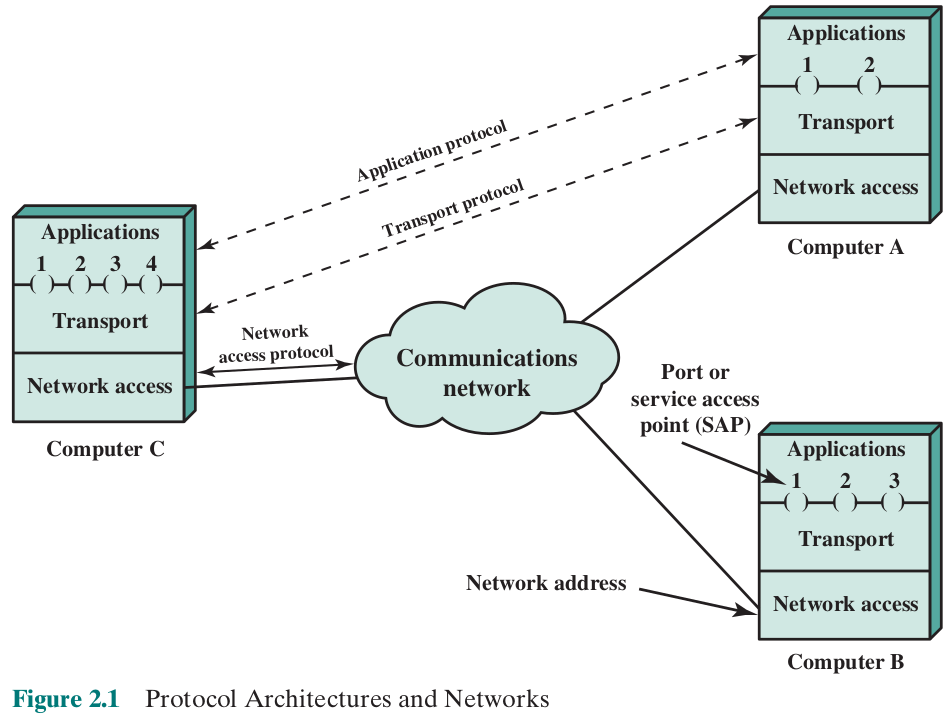
\includegraphics[width=0.8\linewidth]{img/img01}
	\end{center}
\end{frame}

\begin{frame}
	\begin{center}
		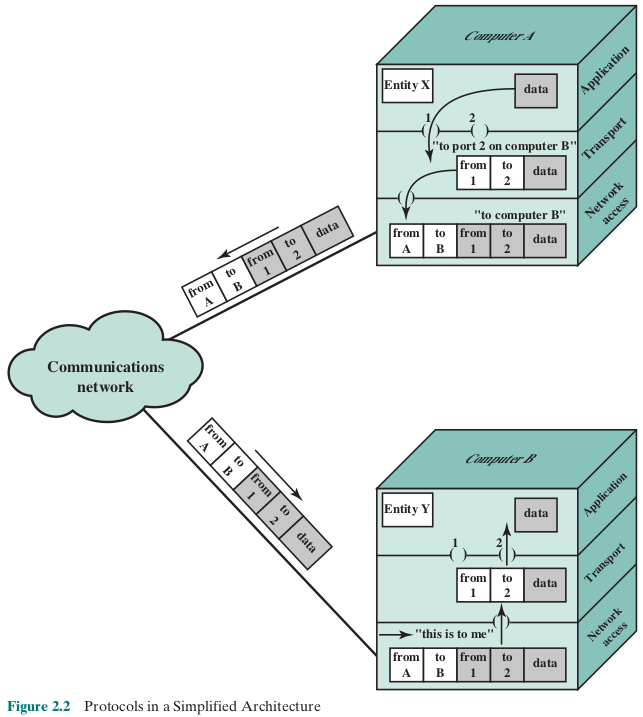
\includegraphics[height=0.9\textheight]{img/img02}
	\end{center}
\end{frame}

\begin{frame}
	\frametitle{TCP/IP Protocol Architecture}
	\begin{itemize}
		\item Result of protocol research and development conducted on ARPANET
		\item Referred to as TCP/IP protocol suite
		\item TCP/IP comprises a large collection of protocols that are Internet standards
	\end{itemize}
\end{frame}

\begin{frame}
	\begin{center}
		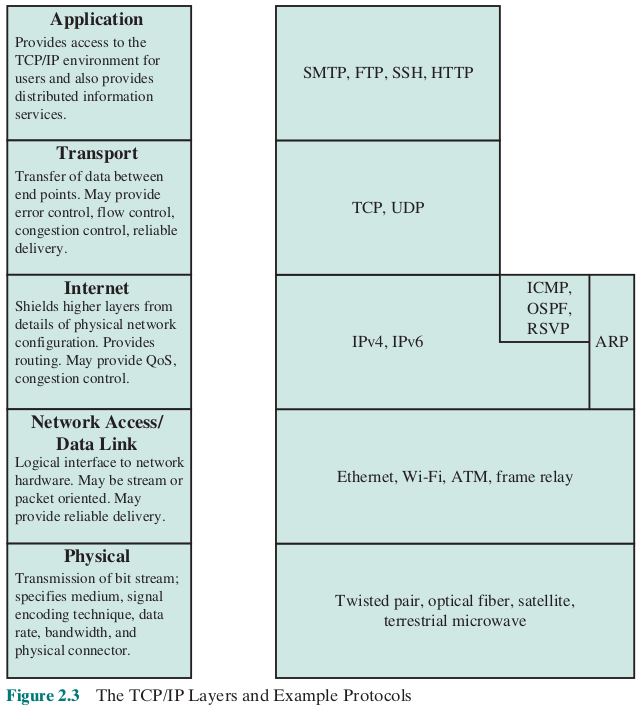
\includegraphics[height=0.9\textheight]{img/img03}
	\end{center}
\end{frame}

\begin{frame}
	\frametitle{Physical Layer}
	\begin{itemize}
		\item Covers the physical interface between computer and network
		\item Concerned with issues like:
		\begin{itemize}
			\item Characteristics of transmission medium
			\item Nature of the signals
			\item Data rates
		\end{itemize}
	\end{itemize}
\end{frame}

\end{document}
